\chapter{Теоретический раздел}

\section{Работа информационного центра}

\subsection*{Режимы работы}

Всего возможно два режима работы информационного центра. 

\begin{itemize}
	\item Режим нормального обслуживания~---~есть свободные операторы, клиент выбирает свободного оператора с максимальной производительностью.
	\item Режим отказа в обслуживании~---~свободных операторов нет, клиенту отказывается в обслуживании.
\end{itemize}

\subsection*{Переменные имитационной модели}

\begin{itemize}
	\item \textbf{Эндогенные переменные}: время обработки задания $i$-ым оператором, время решения задания $j$-ым компьютером.
	\item \textbf{Экзогенные переменные}: число обслуженных клиентов и число клиентов, получивших отказ
\end{itemize}

\subsection*{Уравнения имитационной модели}

\begin{equation}
	P_{\text{отк}} = \frac{C_{\text{отк}}}{C_{\text{отк}} + C_{\text{обсл}}},
\end{equation}

\noindent где $P_{\text{отк}}$~---~вероятность отказа, $C_{\text{отк}}$~---~количество клиентов, которым отказали в обслуживании, $C_{\text{обсл}}$~---~количество клиентов, которым оказали обслуживание.

\newpage

\subsection*{Структурная схема модели}

\begin{figure}[ht]
    \centering
    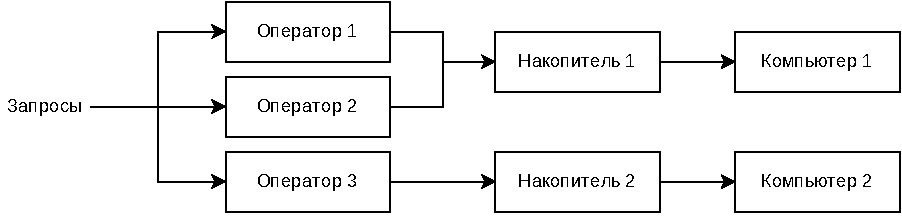
\includegraphics[width=0.8\textwidth]{assets/struct.pdf}
    \caption{Структурная схема модели}
    \label{fig:struct}
\end{figure}

\subsection*{Схема модели в терминах СМО}

\begin{figure}[ht]
    \centering
    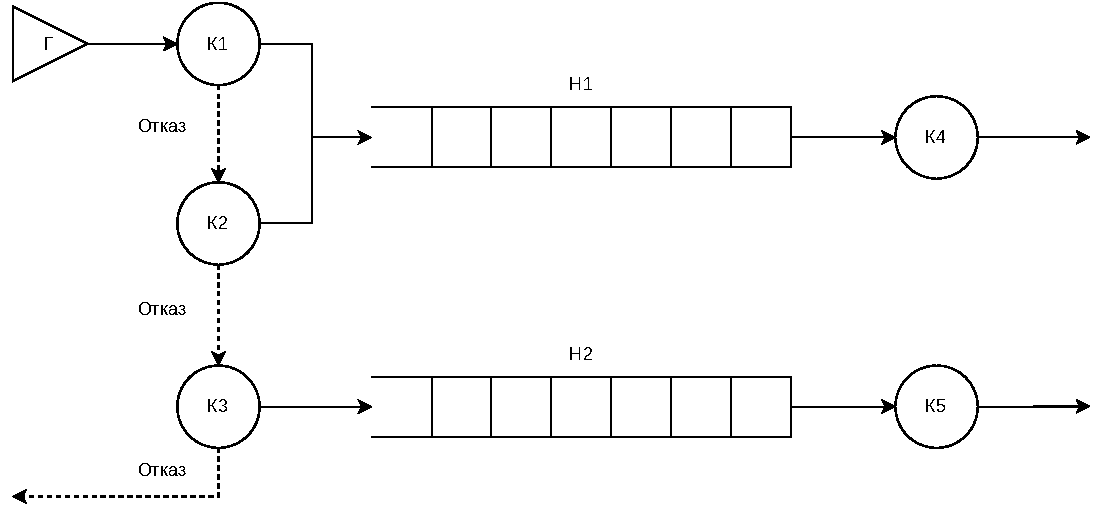
\includegraphics[width=0.8\textwidth]{assets/smo.pdf}
    \caption{Схема модели в терминах СМО}
    \label{fig:smo}
\end{figure}

\section{GPSS}

Система GPSS World~---~мощная универсальная среда моделирования как дискретных, так и непрерывных процессов, предназначенная для профессионального моделирования самых разнообразных процессов и систем. Эта система явилась следующим шагом развития системы GPSS/PC (1984 год), ориентированной на DOS. Обе системы разработаны специалистами фирмы Minuteman Software (основана в 1982 году) под руководством Спрингера Кокса. Сначала система GPSS World появилась в 1994 году с ориентацией на OS/2 фирмы IBM, и только в 2000 году она была реализована под ОС Windows фирмы Microsoft.

С помощью этой системы, например, можно эффективно моделировать как производственные, так и непроизводственные процессы: функционирование торговых и увеселительных заведений, портов, уличное движение, проведение военных действий, работу редакций, учреждений и сети Internet, различных систем массового обслуживания и~т.~д. Система имеет большой набор команд для управления процессом моделирования, которые можно как использовать в интерактивном режиме, так и включать в модель. Обеспечена возможность проведения экспериментов, сгенерированных системой, пользовательских и оптимизационных. В системе GPSSW реализована процедура визуализации процесса функционирования модели с использованием методов мультипликации.

Система GPSSW имеет новый высокоскоростной транслятор, работающий в сотни раз быстрее его предшественников. Для быстрого исправления ошибок используется полноэкранный текстовый редактор.

